\documentclass[tikz, border=5pt]{standalone}
\usetikzlibrary{patterns}

\begin{document}
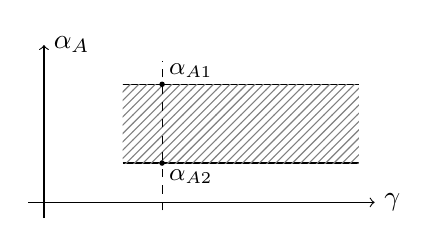
\begin{tikzpicture}

    %% Assignment-2, Q1b

    % Axes
    \draw[->] (-0.2,0) -- (4.2,0) node[right] {\( \gamma \)};
    \draw[->] (0,-0.2) -- (0,2) node[right] {\( \alpha_A \)};

    % Band
    \draw (1,0.5) -- (4,0.5);
    \draw (1,1.5) -- (4,1.5);
    \fill[pattern=north east lines, pattern color=gray] (1,0.5) rectangle (4,1.5);

    % Markings
    \draw[dashed] (1.5,-0.1) -- (1.5,1.8);
    \fill (1.5,1.5) circle (1pt) node[above right=-1] {\small \( \alpha_{A 1} \)};
    \fill (1.5,0.5) circle (1pt) node[below right=-1] {\small \( \alpha_{A 2} \)};

\end{tikzpicture}
\end{document}
